%max: 5pages

\documentclass{llncs}
%
\usepackage{makeidx}  % allows for indexgeneration
\usepackage{graphicx} % for photos
%
\begin{document}
%
\frontmatter          % for the preliminaries
%
\pagestyle{headings}  % switches on printing of running heads
\addtocmark{Hamiltonian Mechanics} % additional mark in the TOC
%

\mainmatter              % start of the contributions
%
\title{Zone-project: towards a better news feed using semantic web}
%
\titlerunning{Zone-project}  % abbreviated title (for running head)
%                                     also used for the TOC unless
%                                     \toctitle is used
%
\author{Christophe Desclaux\inst{1}}
%
\authorrunning{Christophe Desclaux} % abbreviated author list (for running head)
%
%%%% list of authors for the TOC (use if author list has to be modified)
\tocauthor{Christophe Desclaux}
%
\institute{Wimmics Inria, Sophia Antipolis...,\\
\email{christophe@zouig.org},\\ WWW home page:
\texttt{http://www.zone-project.org}
}

\maketitle

\begin{abstract}%
The zone project proposes an innovative solution to address the traditional issues of news feed management using the resources of Semantic Web to group related informations together.
It provides a new way to follow feeds by aggregating items from various RSS feeds, tagging and annotating each one of them. Those tags then provide a basis for filters allowing users to see only relevant news.


%The abstract should summarize the contents of the paper
%using at least 70 and at most 150 words. It will be set in 9-point
%font size and be inset 1.0 cm from the right and left margins.
%There will be two blank lines before and after the Abstract. \dots
\keywords{linked data, data aggregation, RSS}
\end{abstract}
%
\section{Motivation}
%
A lot of news are published every day on the internet and the number of news websites has increased significantly. People and organizations are now building news aggregators in order to filter and sort all this information.

Solutions exist, for instance one can use \textsl{Google news} \footnote{\url{http://news.google.fr}} like a trusted provider of information, but in this web application your are only a consumer and you don't have a lot of interactions with the system. 

A second kind of solutions is to make news forecasting using for instance \textsl{Twitter}\footnote{\url{http://www.twitter.com}}. It's a solution in which one can control the sources he follows. But you can't select precisely on sources and on topics at the same time and a lot of noise remains around good information. Even the hash-tags provide a limited solution since they suffer from collision.  
***************** oui, les recherches par mots tags ne permettent pas de supprimer les bruit liés à l'utilisation de mêmes hashtags sur différents sujets distincts **************************


The last family of relevant solutions one can use is aggregators like \textsl{Yahoo Pipes} \footnote{\url{http://pipes.yahoo.com/pipes/}}. This tool allows the mixing of popular data feeds to create data filtering via a visual editor. It uses pipes as workflows which will help users sort feeds.

From these three types of approaches we can identify some main challenges that good aggregators need to work on:
\begin{itemize}
  \item \textbf{filtering capacities}: we need to be able to select and sort information according to precise criteria.
  \item \textbf{open pool of sources}: the tool needs to have access to a maximum of news present on internet and allow the user to add new ones.
  \item \textbf{independence}: users need to use the solution independently of any provider.
\end{itemize}

Technicals solutions exists in order to solve these challenges. Google solves the filtering problem using [article de Larry Page sur l'aggregation par mots clés] but this solution is not very efficient because it works on words instead of working on meaning. The solution we propose is an aggregation based on semantic web frameworks. 

We will first present in this article our solution called Zone. We will explain the annotation workflow, the ontology used and the use of data-mining solutions. We will also present the script of the demonstration of the application.

%
\section{Application: Zone}


\subsection{the workflow}
%
\begin{figure}[htb!]
	\begin{centering}
	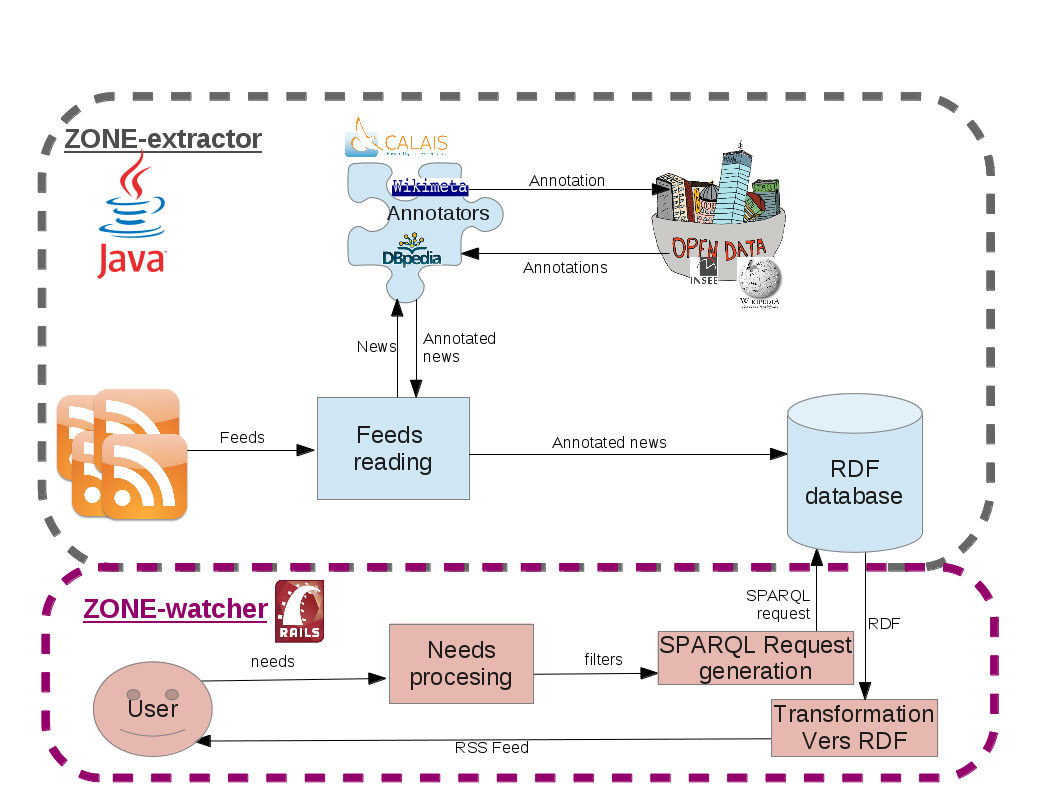
\includegraphics[width=1\textwidth]{diagramArchi.png}
	\caption{Annotation workflows and semantic filtering of news}
	\label{fig:WF}
	\end{centering}
\end{figure}

In order to have a more efficient news selection according to their semantic relevance, we have created two kinds of workflows. Figure \ref{fig:WF} shows the general architecture: a semantic annotation workflow of news and a filtering workflow. The distinction between the two workflows is extremely important in order to work in an asynchronous way.


\subsubsection{The semantic annotation workflow}
First, Zone crawls the web extracting all news and storing them in database.
Two annotators extract semantic annotations from the textual content of the news: one calls Wikimeta to create links to Wikipedia resources and the other calls OpenCalais takes care of the geographical references.
New content and semantic annotations are then stored together in a triple store (Vituoso).

\subsubsection{The filtering workflow}
Zone gives the user the possibility to access all data organized by the annotation workflow. It is designed as a web application using the web framework RubyOnRails \footnote{\url{http://rubyonrails.org}}. Starting from news samples the user can build filters that are stored and applied as SPARQL queries. These queries are then performed over the triple store fed by the annotation workflow. From these selection queries the user can publish an RSS feed of results.

%
\subsection{The Zone News Ontology}
%

% link to other news ontologies
% // event media ontology etc.

% graph of the ontology
% publish on ns.inria.fr 
% textual description of core classes and properties.

**************basée sur RSS
on a ajouté un schéma RDFs spécialisé
on se base aussi sur l'ontologie de wikimeta/insee***************
%

%
\subsection{Using generalisators}
*******parler de l'insee********
Currently the generalisators focus on saturating the annotations with the transitive closure of geographical inclusion (e.g. from an annotation insee:Paris we will add insee:France). 
In the future we intend to add ...
%TODO: add other completions
 

%
\subsection{Using datamining}
section d'Ameni

\section{Demonstration}
%
The web application is designed for all kinds of news feeds be them about technology, medicine or general news. You can install the application according to your needs under the AGPL licence. We also propose a public service for general news feed at \url{http://demo.zone-project.org} which is the main test platform for the application.

The demo will start with the listing of all recent news on \url{http://demo.zone-project.org}. Then we will create a filter according to some criteria in order to show to the audience the different kinds of filters present and their links to the news. Once the good filter is chosen, we will show how to export it as an external RSS feed aggregator demonstrating that our web application can be used in combination to other tools.

Then we will propose another usage of ZONE-project this time based on Twitter. With another demo application we will make a quick demonstration of news filtering on the hashtag #eswc2013.

\section{Conclusion and future work}
%
Challenges qui restent à résoudre :
	*tech : faire des liens vers openData et du raisoning
	*com : trouver moyen de pérenniser le projet
%

\section{Acknowledgments}
%
This project has been started in 2011 according to an and of ingeneering school project and has been 
Description du contexte de travail=> se passe à l'inria BYC... équipe wimmics qui bosse sur semantic web

%





%
% ---- Bibliography ----
%
\begin{thebibliography}{5}
%
\bibitem {clar:eke}
Clarke, F., Ekeland, I.:
Nonlinear oscillations and
boundary-value problems for Hamiltonian systems.
Arch. Rat. Mech. Anal. 78, 315--333 (1982)

\bibitem {clar:eke:2}
Clarke, F., Ekeland, I.:
Solutions p\'{e}riodiques, du
p\'{e}riode donn\'{e}e, des \'{e}quations hamiltoniennes.
Note CRAS Paris 287, 1013--1015 (1978)

\bibitem {mich:tar}
Michalek, R., Tarantello, G.:
Subharmonic solutions with prescribed minimal
period for nonautonomous Hamiltonian systems.
J. Diff. Eq. 72, 28--55 (1988)

\bibitem {tar}
Tarantello, G.:
Subharmonic solutions for Hamiltonian
systems via a $\bbbz_{p}$ pseudoindex theory.
Annali di Matematica Pura (to appear)

\bibitem {rab}
Rabinowitz, P.:
On subharmonic solutions of a Hamiltonian system.
Comm. Pure Appl. Math. 33, 609--633 (1980)

\end{thebibliography}

\clearpage
\end{document}